\documentclass[onecolumn]{article}
%\usepackage{url}
%\usepackage{algorithmic}
\usepackage[a4paper]{geometry}
\usepackage{datetime}
\usepackage[margin=2em, font=small,labelfont=it]{caption}
\usepackage{graphicx}
\usepackage{mathpazo} % use palatino
\usepackage[scaled]{helvet} % helvetica
\usepackage{microtype}

\usepackage{multicol}
\usepackage{amsmath}
\usepackage{subfigure}
\usepackage{comment}
% Letterspacing macros
\newcommand{\spacecaps}[1]{\textls[200]{\MakeUppercase{#1}}}
\newcommand{\spacesc}[1]{\textls[50]{\textsc{\MakeLowercase{#1}}}}

\title{\spacecaps{Final Report}\\ \normalsize \spacesc{CENG 3521, Data Mining} }

\author{Edanur Pişkin - Yiming Aijiaerguli \\edanurpiskin@posta.mu.edu.tr - 170709509@posta.mu.edu.tr}
%\date{\today\\\currenttime}
\date{\today}

\begin{document}
\maketitle

\begin{abstract}
House prices were estimated in this study with AmesHouse dataset. Data had many missing values. These missing values were filled by various methods. Then, the data set that gave us the best result was prepared. Different models were used, namely linear regression and MLP. Results were compared according to the RMSE and R-squared values. The results obtained at the end of the study were satisfying.
\end{abstract}

\section{Introduction}

In this project, it is aimed to predict house prices by using house features. Prediction performance has been tried to be increased by using different methods such as feature selection, outlier detection and scaling. The missing data were filled by examining the categorical and numerical variables in detail. Various visualization methods have been used to select the features which will give best results. Features were examined in detail and their effects on the price were observed. Linear regression is used as the estimation algorithm. As the last step, all results are compared with each other. Algorithm and data that give the best result are determined.

\section{Project Details}

\subsection{Data}

Ames House Dataset was selected for the house price estimation project. The data includes 2930 different houses and 82 features in total. The columns are as follows.

\begin{multicols}{3}
\noindent \footnotesize{SalePrice - the property's sale price in dollars. This is the target variable that you're trying to predict.
\\MSSubClass: The building class
\\MSZoning: The general zoning classification
\\LotFrontage: Linear feet of street connected to property
\\LotArea: Lot size in square feet
\\Street: Type of road access
\\Alley: Type of alley access
\\LotShape: General shape of property
\\LandContour: Flatness of the property
Utilities: Type of utilities available
\\LotConfig: Lot configuration
\\LandSlope: Slope of property
\\Neighborhood: Physical locations within Ames city limits
\\Condition1: Proximity to main road or railroad
\\Condition2: Proximity to main road or railroad (if a second is present)
\\BldgType: Type of dwelling
\\HouseStyle: Style of dwelling
\\OverallQual: Overall material and finish quality
\\OverallCond: Overall condition rating
\\YearBuilt: Original construction date
\\YearRemodAdd: Remodel date
\\RoofStyle: Type of roof
\\RoofMatl: Roof material
\\Exterior1st: Exterior covering on house
\\Exterior2nd: Exterior covering on house (if more than one material)
\\MasVnrType: Masonry veneer type
\\MasVnrArea: Masonry veneer area in square feet
\\ExterQual: Exterior material quality
\\ExterCond: Present condition of the material on the exterior
\\Foundation: Type of foundation
\\BsmtQual: Height of the basement
\\BsmtCond: General condition of the basement
\\BsmtExposure: Walkout or garden level basement walls
\\BsmtFinType1: Quality of basement finished area
\\BsmtFinSF1: Type 1 finished square feet
\\BsmtFinType2: Quality of second finished area (if present)
\\BsmtFinSF2: Type 2 finished square feet
\\BsmtUnfSF: Unfinished square feet of basement area
\\TotalBsmtSF: Total square feet of basement area
\\Heating: Type of heating
\\HeatingQC: Heating quality and condition
\\CentralAir: Central air conditioning
\\Electrical: Electrical system
\\1stFlrSF: First Floor square feet
\\2ndFlrSF: Second floor square feet
\\LowQualFinSF: Low quality finished square feet (all floors)
\\GrLivArea: Above grade (ground) living area square feet
\\BsmtFullBath: Basement full bathrooms
\\BsmtHalfBath: Basement half bathrooms
\\FullBath: Full bathrooms above grade
\\HalfBath: Half baths above grade
\\Bedroom: Number of bedrooms above basement level
\\Kitchen: Number of kitchens
\\KitchenQual: Kitchen quality
\\TotRmsAbvGrd: Total rooms above grade (does not include bathrooms)
\\Functional: Home functionality rating
\\Fireplaces: Number of fireplaces
\\FireplaceQu: Fireplace quality
\\GarageType: Garage location
\\GarageYrBlt: Year garage was built
\\GarageFinish: Interior finish of the garage
\\GarageCars: Size of garage in car capacity
\\GarageArea: Size of garage in square feet
\\GarageQual: Garage quality
\\GarageCond: Garage condition
\\PavedDrive: Paved driveway
\\WoodDeckSF: Wood deck area in square feet
\\OpenPorchSF: Open porch area in square feet
\\EnclosedPorch: Enclosed porch area in square feet
\\3SsnPorch: Three season porch area in square feet
\\ScreenPorch: Screen porch area in square feet
\\PoolArea: Pool area in square feet
\\PoolQC: Pool quality
\\Fence: Fence quality
\\MiscFeature: Miscellaneous feature not covered in other categories
\\MiscVal: \$Value of miscellaneous feature
\\MoSold: Month Sold
\\YrSold: Year Sold
\\SaleType: Type of sale
\\SaleCondition: Condition of sale}

\end{multicols}


\subsection{Handling Missing Values}
27 columns have missing values. Details of missing value are shown in Figure 1. Since some of the features have many missing values, deleting missing values will not be the right method. Different methods are used for categorical and numerical missing values. For categorical data, missing values show that the house does not have that feature. Therefore, the missing values are filled in as "does not have feature". Two ways can be used to fill in numerical data. Missing values can be filled by mean and median. However, it is necessary to decide which method should be used for each feature. To decide which method will be used, it is necessary to examine the distribution of columns with missing values. Two ways can be used to fill in numerical data. Missing values can be filled by mean and median. However, it is necessary to decide which method should be used for each feature. To decide which method will be used, distribution of columns  with missing values needs to be examined. See Figure 3. Distributions which are similar to the normal distribution can be filled with mean value. But if the distribution is skewed, it should be filled with median value. When the plot is examined, it is seen that the LotFrontage feature is similar to the normal distribution, while the MasVnrArea and GarageYtBlt features are skewed. The missing values in LotFrontage will be imputed by the mean value and missing values in MasVnrArea and GarageYrBlt features will be imputed by the median value. 



\begin{figure}[h]
\centering
\begin{minipage}{.3\textwidth}
  \centering
  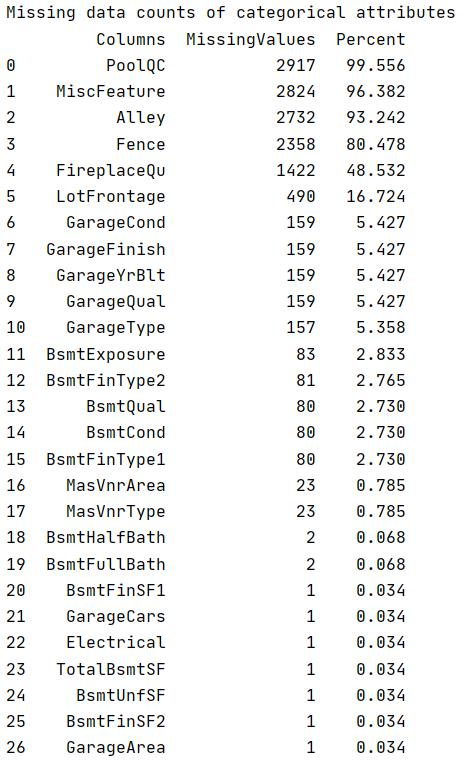
\includegraphics[width=.9\linewidth]{missing_values.jpg}
  \captionof{figure}{Missing Values}
  \label{fig:missing_values}
\end{minipage}%
\begin{minipage}{.7\textwidth}
  \centering
  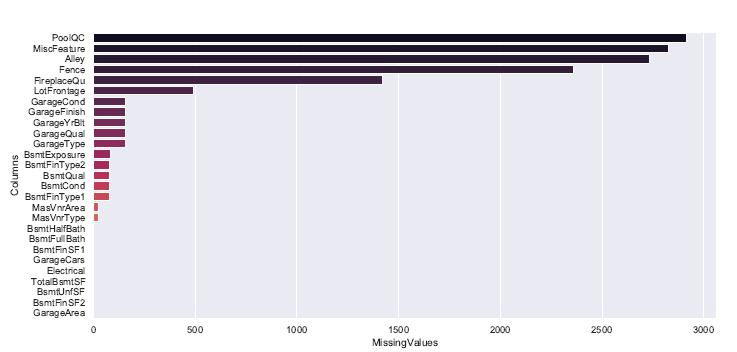
\includegraphics[width=.9\linewidth]{missing_values_2.jpg}
  \captionof{figure}{Missing Values Plot}
  \label{fig:missing_values_2}
\end{minipage}
\end{figure}


\begin{figure}[h]
\centering
  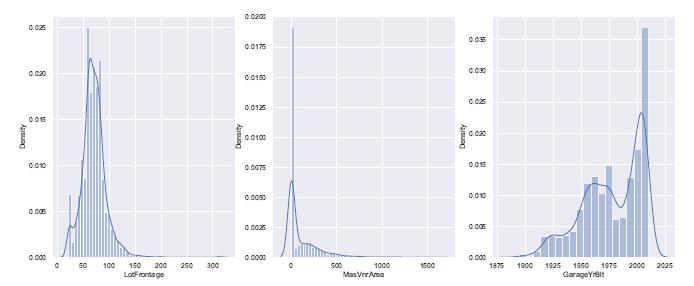
\includegraphics[width=0.6\linewidth]{distribution.jpg}
  \caption{Distribution Of Attributes With Missing Values}
  \label{fig:distribution}
\end{figure}


\subsection{Binarization}

Categorical data should be binarized to use data in regression analysis. After binarization, the data increased from 82 columns to 275 columns. One hot encoding is used.

\subsection{First Regression Analysis}
First of all, regression analysis was applied without any improvement of dataset. This result is taken as the base result. The results of other regressions will be compared with this base result. Before applying regression, it is necessary to fit the attribute which will be predicted to the normal distribution. For this, the log of the sales price is used. The graphs of the distributions are also shown below. See Figure 4. Then regression analysis is applied. R-squared and RMSE are used as performance measurement metrics. R-squared is a statistical measure of how close the data are to the fitted regression line. Root mean squared error (RMSE) is the square root of the mean of the square of all of the error. The results are shown below.\\
\textit{R-squared : 0.82\\
RMSE: 0.17}\\
Results are not bad but can be improved. The plot in Figure 5 shows the scatter plot of actual values and predicted values.


\begin{figure}[h]
\centering
\begin{minipage}{.6\textwidth}
  \centering
  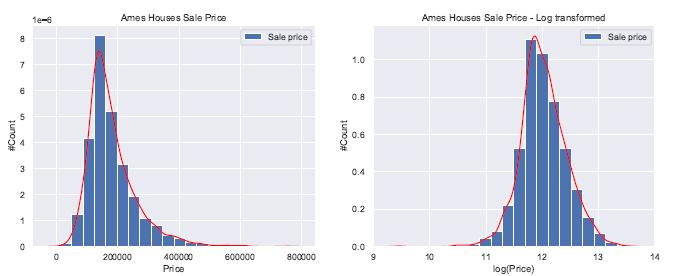
\includegraphics[width=.9\linewidth]{distribution_2.jpg}
  \captionof{figure}{SalePrice – Log Transformed SalePrice}
  \label{fig:distribution_2}
\end{minipage}%
\begin{minipage}{.4\textwidth}
  \centering
  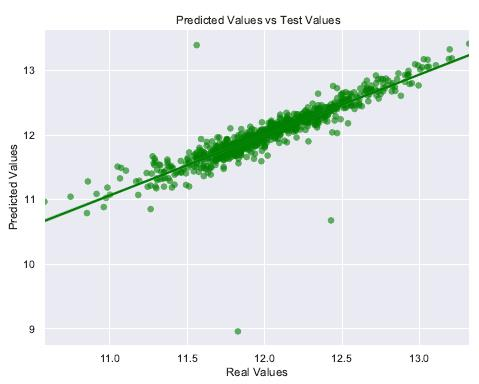
\includegraphics[width=.9\linewidth]{non_featured.jpg}
  \captionof{figure}{Non-featured Regression Plot}
  \label{fig:non_featured}
\end{minipage}
\end{figure}


\subsection{Outliers}
Boxplot of sale price attribute are examined to detect outliers. Values outside 1.5 IQR value are assumed to be outlier. See Figure 6. Outlier values were filtered and regression was applied again. Results are given below.\\
\textit{R-squared: 0.77\\
RMSE: 0.19}\\
R-squared value decreased and RMSE value is increased. These results are worse than our base results. For these reasons, it is decided to keep the outliers.


\begin{figure}[h]
\centering
  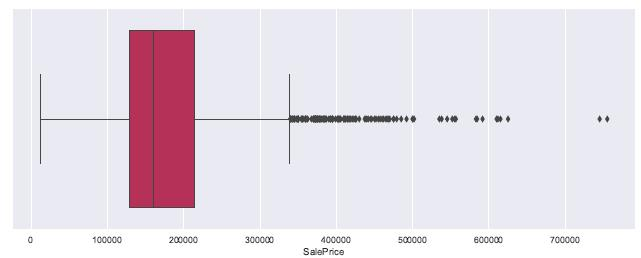
\includegraphics[width=0.6\linewidth]{box_saleprice.jpg}
  \caption{Box plot of SalePrice}
  \label{fig:box_saleprice}
\end{figure}

\subsection{Feature Selection}
In order to determine the most important numerical features for prediction, the correlation between the features with each other and with the sales price was examined. See Figure 7. Boxplots of some of the most important features are shown in Figure 11. Boxplot was used to determine the most important square features. When the plot is examined, it is seen that some features are more correlated with the sales price than others. First 10 numeric properties with the highest correlation were used. Plot shown in Figure 9 shows the correlation between the selected most important features. When the results were examined, it can be seen that the overall quality, living area square feet, garage area, basement square feet, first floor square feet, built year, bathroom count, remodel date and garage built year were the most effective features on the price of the house. Boxplots were examined to select the most important categorical features. Those with significant differences between values identified as the most important categorical features.\\
Regression was applied again with these selected data. Results is shown below and graph is shown in Figure 10.\\
\textit{R-squared : 0.92\\
RMSE: 0.12}\\
When the results were examined, it was seen that a better result was obtained compared to the result selected as the base. It has been decided to continue with only important features.

\begin{figure}[h]
\centering
\begin{minipage}{.6\textwidth}
  \centering
  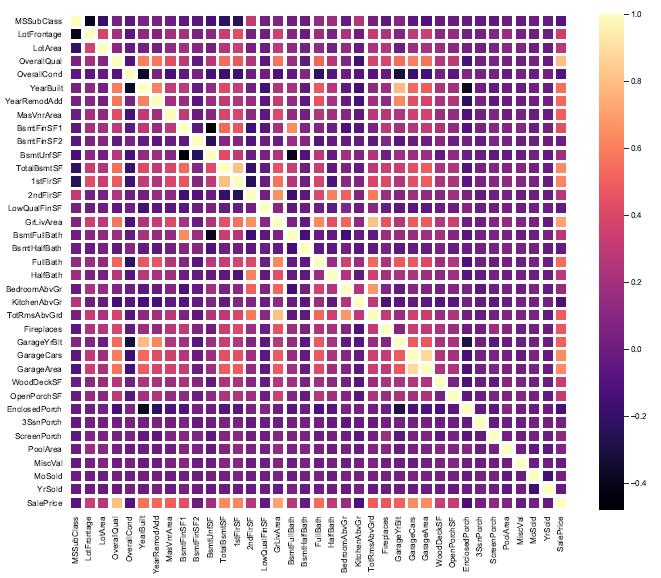
\includegraphics[width=.7\linewidth]{correlation.jpg}
  \captionof{figure}{Correlations}
  \label{fig:correlation}
\end{minipage}%
\begin{minipage}{.4\textwidth}
  \centering
  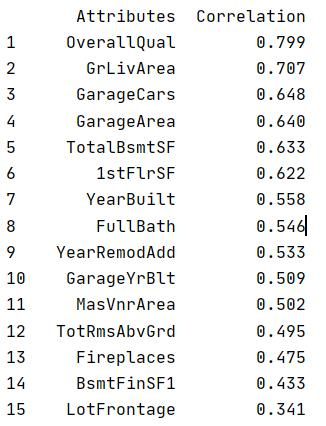
\includegraphics[width=.7\linewidth]{corr_output.jpg}
  \captionof{figure}{Correlation}
  \label{fig:corr_output}
\end{minipage}
\end{figure}

\begin{figure}[h]
\centering
\begin{minipage}{.5\textwidth}
  \centering
  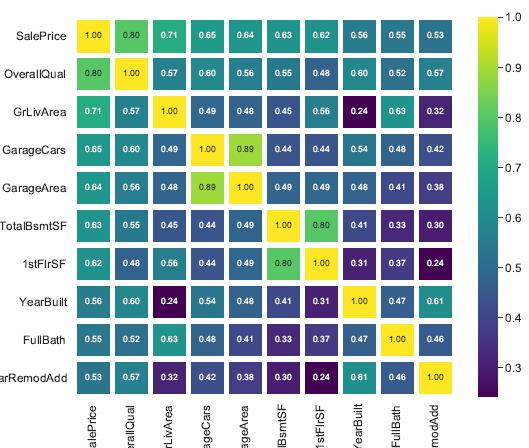
\includegraphics[width=.7\linewidth]{corr_important.jpg}
  \captionof{figure}{Correlation Between Most Important Features}
  \label{fig:corr_important}
\end{minipage}%
\begin{minipage}{.5\textwidth}
  \centering
  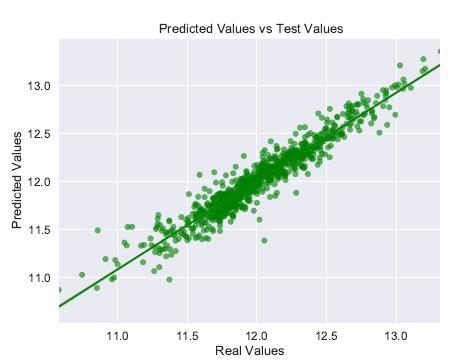
\includegraphics[width=.7\linewidth]{feature_sel_reg.jpg}
  \captionof{figure}{Feature Selection Regression Plot}
  \label{fig:feature_sel_reg}
\end{minipage}
\end{figure}


\begin{figure}[h]
\centering
  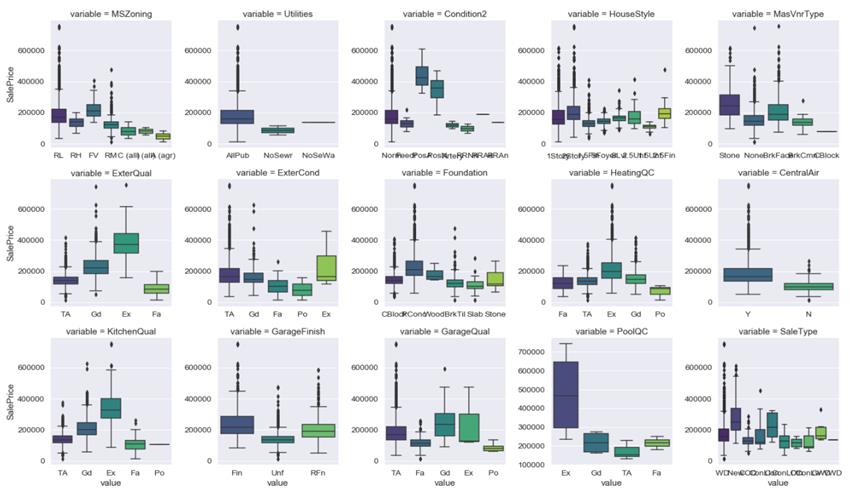
\includegraphics[width=0.7\linewidth]{boxplot_important.jpg}
  \caption{Box Plots of Most Important Categorical Attributes}
  \label{fig:boxplot_important}
\end{figure}

\subsection{Scaling}
Standard scaler is used to scale the data. Then regression was applied with scaled data. Because of randomness result may differ. The results are shown below.\\ 
\textit{R-squared : -227\\
RMSE: 6.04\\}
After feature selecting, most of the data are categorical. For this reason, scaling did not have a positive effect on regression results. R-squared values is decreased and RMSE is increased.

\subsection{MLP Regression}
Finally, MLP regression is applied. It has been tested whether it will give better results than linear regression. The result is stated below.\\
\textit{R-squared : -0.59\\
RMSE: 0.5\\}
The results obtained are worse than linear regression.


\section{Results}

4 different prediction models have been established. In the first model, all features were used without making any change in the data. Then outliers were determined and removed from the data. Since our data has many different features, the important ones among these features were selected and the regression model was established. Finally, MLP regression model is established. The R-squared and RMSE values of these models were calculated. The results obtained is shown below. When the results are examined, it is seen that the best result is linear regression. Outlier detection did not affect performance positively. The data that gives the best results is the data filtered with feature selection methods.

\begin{figure}[h]
\centering
  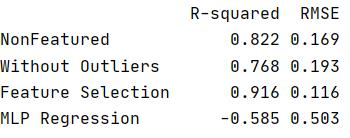
\includegraphics[width=0.4\linewidth]{result.jpg}
  \caption{Result}
  \label{fig:result}
\end{figure}

\section{Conclusion}

Many data preparation methods and different prediction models are applied. When the results were examined, it was decided to use linear regression. The data set that gives the best result is the data prepared with the feature selection method. The features that affect house prices the most were determined. When the results are examined, it is seen that model can explain the variation of the data by 92\%. 


































\nocite{*}
\bibliographystyle{plain}
\bibliography{references}
\end{document}

